\documentclass[letterpaper, twoside, 12pt]{book}

\usepackage{amsmath,amsfonts, amsthm}
\usepackage{yfonts}
\usepackage{amsrefs}
\usepackage{fancyhdr}
\usepackage{graphicx}
\usepackage{float}
\usepackage[margin=1in]{geometry}
\usepackage{array}
\usepackage{esint}
\usepackage{harpoon}
\usepackage{stmaryrd}
\usepackage{multicol}
\usepackage{multirow}
\usepackage{pgf,tikz}
\usetikzlibrary{arrows}

\usepackage{makeidx}
\makeindex

\definecolor{AuburnOrange}{RGB}{221,85,12}
\definecolor{AuburnBlue}{RGB}{3,36,77}
\definecolor{AuburnSecondaryBlue}{RGB}{73,110,156}
\definecolor{AuburnSecondaryOrange}{RGB}{246,128,38}
\definecolor{AlabamaCrimson}{RGB}{163,38,65}
\definecolor{LSUpurple}{RGB}{70,29,124}
\definecolor{VanderbiltGold}{RGB}{207,181,59}

\usepackage[pdfpagelabels]{hyperref}
\hypersetup{colorlinks=true,linkcolor=AuburnSecondaryOrange}

% \usepackage[tracking]{microtype}
% \UseMicrotypeSet{all}
% \SetTracking[spacing = {35*,0*,0*}]{encoding = *}{7}
% \linespread{1.025}

\def\scaleint#1{\vcenter{\hbox{\scaleto[3ex]{\displaystyle\int}{#1}}}}
\def\bs{\!\!}

\renewcommand{\arraystretch}{1.5}

\pagestyle{fancy} \headheight 14.49998pt

\newcommand{\tstamp}{\today}
\renewcommand{\chaptermark}[1]{\markboth{#1}{}}
\renewcommand{\chaptermark}[1]{\markright{#1}}

\lhead[\fancyplain{}{Clontz \thepage}]         {\fancyplain{}{\scshape\nouppercase{\rightmark}}}

\chead[\fancyplain{}{}]
{\fancyplain{}{}}


\rhead[\fancyplain{}{Calculus II Lecture Notes}]       {\fancyplain{}{Clontz \thepage}}

\lfoot[\fancyplain{}{Auburn University}]                 {\fancyplain{\tstamp}{\tstamp}}

\cfoot[\fancyplain{\thepage}{}]         {\fancyplain{\thepage}{}}

\rfoot[\fancyplain{\tstamp} {\tstamp}]  {\fancyplain{}{Auburn University}}

\theoremstyle{definition}
\newtheorem{theorem}{Theorem}

% \theoremstyle{plain}
\newtheorem{proposition}[theorem]{Proposition}
\newtheorem{recall}[theorem]{Recall}

\theoremstyle{definition}
\newtheorem{definition}[theorem]{Definition}
\newtheorem{notation}[theorem]{Notation}
\newtheorem{goal}[theorem]{Goal}
\newtheorem{motivation}[theorem]{Motivation}
\newtheorem{remark}[theorem]{Remark}
\newtheorem{TrueFact}[theorem]{True Fact}
\newtheorem{FalseFact}[theorem]{False Fact}
\newtheorem{conjecture}[theorem]{Conjecture}
\newtheorem{conclusion}[theorem]{Conclusion}
\newtheorem{observation}[theorem]{Observation}
\newtheorem{problem}[theorem]{Problem}
\newtheorem{question}[theorem]{Question}
\newtheorem{example}[theorem]{Example}
\newtheorem{note}[theorem]{Note}
\newtheorem{convention}[theorem]{Convention}
\newtheorem{eqn}[theorem]{Equation}
\newtheorem{strategy}[theorem]{Strategy}
\newtheorem{properties}[theorem]{Properties}
\newtheorem{corollary}[theorem]{Corollary}

\newcommand{\HRule}{\rule{\linewidth}{0.5mm}}
\newcommand{\harpvec}[1]{\overrightharp{\ensuremath{\mathbf{#1}}}}
\newcommand*{\threevec}[3]{\ensuremath{\left\langle #1, #2, #3 \right\rangle}}
\newcommand*{\twovec}[2]{\ensuremath{\left\langle #1, #2 \right\rangle}}
\newcommand*{\unitvec}[1]{\ensuremath{\mathbf{\widehat{#1}}}}
\newcommand{\veci}{\ensuremath{\mathbf{\widehat{i}}}}
\newcommand{\vecj}{\ensuremath{\mathbf{\widehat{j}}}}
\newcommand{\veck}{\ensuremath{\mathbf{\widehat{k}}}}
\newcommand{\ds}{\ensuremath{\displaystyle}}


\newcommand{\contrasymb}{\mathrel{\raisebox{.1em}{\reflectbox{\rotatebox[origin=c]{220}{$\lightning$}}}}}

\newenvironment{answer}{\paragraph{Answer.}}{\hfill$\blacklozenge$}
\newenvironment{contraproof}{\paragraph{Proof.}}{\hfill$\contrasymb$}

\begin{document}

\setcounter{chapter}{5}

\chapter{Applications of Integrals}

\section{Area Between Curves}

\subsection{Area with Respect to the \emph{x}-axis}

\begin{recall}
  If $f(x)$ is a continuous function and $a\leq b$, then
  the definite integral $\ds\int_a^b f(x)\,dx$ represents the ``net area''
  between the curve $y=f(x)$ and the $x$-axis between $x=a$ and $x=b$.
  (``Net area'' means the area above the $x$-axis minus the area below
  the $x$-axis.)
\end{recall}

\begin{theorem}\index{Area Between Functions of $x$}
  If $f,g$ are continuous functions of $x$ such that $f(x)\leq g(x)$ for all
  $a\leq x\leq b$, then the area $A$ of the region bounded by the curves
  $y = f(x)$, $y = g(x)$, $x = a$, and $x = b$ is
  \[
    A = \int_a^b g(x) - f(x) \, dx
  \]
\end{theorem}

\begin{problem}
 Find the area of the region bounded above by $y = e^x$, below by $y = x$,
 and on the sides by $x = 0$ and $x = 1$.
\end{problem}

\newpage

\begin{problem}
 Find the area bounded by $y = x^2$ and $y = 2x-x^2$.
\end{problem}

\vfill

\begin{problem}
 Find the area bounded by $y = \sin(x)$ and $y = \cos(x)$ from $x = 0$ to
 $x = \frac{\pi}{2}$.
\end{problem}

\vfill

\newpage

\subsection{Area with Respect to the \emph{y}-axis}

\begin{theorem}\index{Area Between Functions of $y$}
  If $f,g$ are continuous functions of $y$ such that $f(y)\leq g(y)$ for all
  $c\leq y\leq d$, then the area $A$ of the region bounded by the curves
  $x = f(y)$, $x = g(y)$, $y = c$, and $y = d$ is
  \[
    A = \int_c^d g(y) - f(y) \, dy
  \]
\end{theorem}

\begin{problem}
 Find the area enclosed by $y = x-1$ and $y^2 = 2x+6$.
\end{problem}

\vfill

\begin{problem}
 Find the area enclosed by $x = 2y-y^2$ and $x = y^2-4y$.
\end{problem}

\vfill

\noindent Suggested Homework: Section $6.1$ numbers
  $1,$ $4,$ $12,$ $24,$ $27,$ $44,$ $50$

\newpage

\section{Volumes by Cross-Sections}

\begin{definition}
  The three-dimensional solid obtained by moving a planar shape
  along a line perpendicular to the plane is called a \textbf{cylinder}.
\end{definition}

\begin{definition}\index{Volume of Cylinder}
  The volume $V$ of a cylinder with base area $B$ and height $h$ is defined
  to be
  \[
    V = Bh
  \]
\end{definition}

\begin{definition}\index{Volume of Solid}
  The volume of a solid positioned between $x=a$ and $x=b$ with cross-sectional
  areas given by $A(x)$ for each $x$-value between $a$ and $b$ is defined to be
  \[
    V
      =
    \lim_{n\to\infty} \sum_{i=1}^n A(x_{i,n})\,\Delta x_n
      =
    \int_a^b A(x)\,dx
  \]
\end{definition}

\begin{problem}
  Show that the volume $V$ of a pyramid with height $h$
  and a square base with side length $s$ is $\ds V = \frac{1}{3}s^2h$.
\end{problem}

\vfill

\newpage

\begin{definition}
  A \textbf{solid of revolution} is the result of rotating a shape around
  a line (called the \textbf{axis of revolution}).
\end{definition}

\begin{theorem}[Disc Method\index{Disc Method}]
  Suppose that a solid of revolution is formed from a shape positioned flush
  against a horizontal or vertical axis of revolution.

  If the axis of revolution is horizontal, and $R(x)$ gives the distance from the
  axis to the outside of the shape being rotated for each value of $x$,
  then the volume of the solid of revolution from $x=a$ to $x=b$ is
  \[
    V = \int_a^b \pi [R(x)]^2\, dx
  \]
  If the axis of revolution is vertical, and $R(y)$ gives the distance from the
  axis to the outside of the shape being rotated for each value of $y$,
  then the volume of the solid of revolution from $y=c$ to $y=d$ is
  \[
    V = \int_c^d \pi [R(y)]^2\, dy
  \]
\end{theorem}

\begin{problem}
 Show that the volume of a sphere of radius $r$ is $\ds V = \frac{4}{3}\pi r^3$.
\end{problem}

\vfill

\newpage

\begin{problem}
 Find the volume of the solid obtained by rotating the shape bounded by
 $y=\sqrt{x}$, $y=0$, $x=0$, and $x=1$ about the $x$-axis.
\end{problem}

\vfill

\begin{problem}
 Find the volume of the solid obtained by rotating the shape bounded by
 $y = x^3$, $x=0$, $y = 0$, and $y=8$ about the $y$-axis.
\end{problem}

\vfill

\newpage

\begin{theorem}[Washer Method\index{Washer Method}]
  Suppose that a solid of revolution is formed from a shape not positioned flush
  against a horizontal or vertical axis of revolution.

  If the axis of revolution is horizontal, $R(x)$ gives the distance from the
  axis to the outside of the shape being rotated for each value of $x$, and
  $r(x)$ gives the distance from the axis to the inside of the shape being
  rotated for each value of $x$,
  then the volume of the solid of revolution from $x=a$ to $x=b$ is
  \[
    V = \int_a^b \pi [R(x)]^2-\pi [r(x)]^2\, dx
  \]
  (The similar formula works for $y$ values and a vertial axis of revolution.)
\end{theorem}

\begin{problem}
 Find the volume of the solid obtained by rotating the triangle with
 vertices at $(1,1)$, $(3,1)$, and $(1,2)$ around the $x$-axis.
\end{problem}

\vfill

\begin{problem}
 Find the volume of the solid obtained by rotating the region bounded by
 $y=x$ and $y=x^2$ about the line $x = -1$.
\end{problem}

\vfill

\noindent Suggested Homework: Section $6.2$ numbers $4,$ $5,$ $12,$ $15,$ $19,$ $25,$ $42,$ $54,$ $56,$ $59$
\newpage

% \section{Volume by Cylindrical Shell}

% \begin{figure}[H]
%  \centering
%  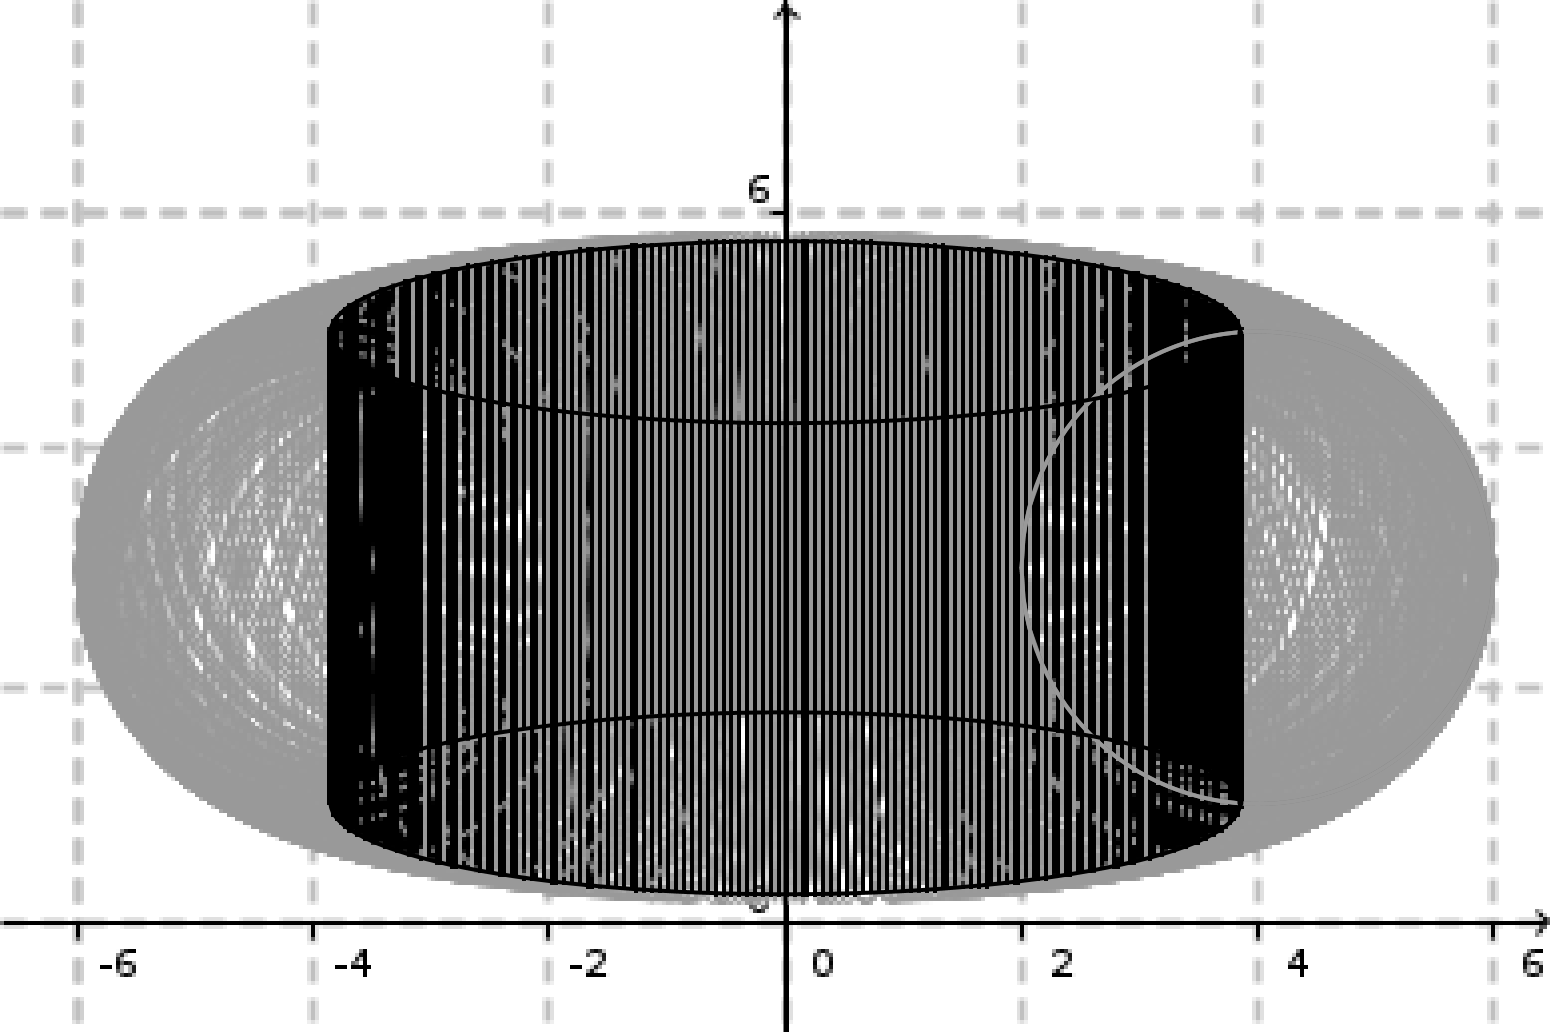
\includegraphics[width=3in]{ShellMethodLectureNotes.png}
%  \caption{Shell Method}
%  \label{ShellMethodFigure}
% \end{figure}

% \begin{motivation}
%  Sometimes it is easier to deal with cylindrical shells rather than discs.  When this happens, what we want to do is peal away sections of this surface one layer at a time, much like layers of an onion (not to be confused with \emph{The Onion}).  In this case, each layer can be straightened out and placed on a table so that it looks like a rectangular prism, which has volume length times width times height.  The length of the shell is the circumference of the shell, the length is the height, and the width is $\Delta x$.  This width will become arbitrarily small with the integration.
% \end{motivation}

% \begin{theorem}[Shell Method\index{Shell Method}]
%  The volume of a solid rotated about the $y$-axis under the curve $y = f(x)$ from $y = a$ to $y = b$ is $V = \int_a^b 2\pi x f(x) \, dx$.
% \end{theorem}

% \begin{problem}
%  Find the volume of the solid obtained by rotating $y = 2x^2-x^3$ and $y = 0$ about the $y$-axis.
% \end{problem}

% \vfill

% \begin{problem}
%  Find the volume of the solid obtained by rotating $y = x$ and $y = x^2$ about the $y$-axis.
% \end{problem}

% \vfill

% \newpage

% \begin{problem}
%  Find the volume of the solid obtained by rotating $y = \sqrt{x}$  about the $x$-axis from $y = 0$ to $y = 1$.
% \end{problem}

% \vfill

% \begin{problem}
%  Find the volume of the solid obtained by rotating $y = x-x^2$ and $y = 0$ about the line $x=2$.
% \end{problem}

% \vfill

% Suggested Homework: Section $6.3$ numbers $2,$ $7,$ $9,$ $17,$ $19,$ $37$

% \newpage

% \setcounter{chapter}{7}

% \chapter{Further Applications of Integrals}

% \section{Arc Length}

% \begin{goal}
%  To find the length of a curve.  That is to say that if there were a peice of string laying right on top of the curve, and we straightened it out, how long would the string be?
% \end{goal}

% \begin{strategy}
%  We will divide the interval we are interested in into $n$ segments, just as we did with Riemann Sums.  Let $P_k$ denote the $k^{\rm th}$ point within the interval we are interested in.  Then the arc Length is $$L = \lim_{n \rightarrow \infty} \sum_{i = 0}^n d\left(P_{i-1}, P_i\right).$$
%  Moreover, let $\Delta y_i = y_i - y_{i-1}.$  Then we can express that distance as
%  $$\begin{array}{rclcl}
%     d\left(P_{i-1}, P_i\right) &=& \sqrt{\left(x_i - x_{i-1}\right)^2 + \left(y_i - y_{i-1}\right)^2}   &=& \sqrt{\left(\Delta x\right)^2 + \left(\Delta y_i\right)^2} \\
%                                &=& \sqrt{\left(\Delta x\right)^2 + \left[f^\prime\left(x_i^*\right)\Delta x\right]^2} &=& \sqrt{1+\left[f^\prime\left(x_i^*\right)\right]^2} \Delta x.
%    \end{array}$$
%  Putting this all together, we have $$L = \lim_{n \rightarrow \infty}\sum_{i=1}^n d\left(P_{i-1},P_i\right) = \lim_{n \rightarrow \infty}\sum_{i=1}^n \sqrt{1+\left[f^\prime\left(x_i^*\right)\right]^2} \Delta x = \int_a^b \sqrt{1+\left[f^\prime\left(x_i^*\right)\right]^2} \Delta x.$$
%  The motivation for this can be seen in Figure \ref{ArcLengthFigure}
% \end{strategy}

% \begin{theorem}[Arc Length\index{Arc Length}]
%  If $f^\prime$ is continuous on $\left[a,b\right]$, then the length of the curve $y = f(x), a \leq x \leq b$ is $$L = \int_a^b \sqrt{1+\left[f^\prime\left(x\right)\right]^2} \, dx.$$
% \end{theorem}

% \begin{figure}[H]
%   \centering

%   \definecolor{yqyqyq}{rgb}{0.50196,0.50196,0.50196}
%   \definecolor{uququq}{rgb}{0.25098,0.25098,0.25098}
%   \begin{tikzpicture}[line cap=round,line join=round,>=triangle 45,x=1.0cm,y=1.0cm]
%   \draw[->,color=black] (0,2.45864) -- (0,10.02955);
%   \foreach \y in {2,3,4,5,6,7,8,9,10}
%   \draw[shift={(0,\y)},color=black] (2pt,0pt) -- (-2pt,0pt) node[left] {\footnotesize $\y$};
%   \clip(-2.85396,2.45864) rectangle (3.49247,10.02955);
%   \draw[smooth,samples=100,domain=-2.8539580190104856:3.492470601051677] plot(\x,{((\x)+0.1)*((\x)+1.1)*((\x)-1.9)+5.1});
%   \draw [line width=2pt,color=yqyqyq] (-1.5,3.196)-- (-0.94286,5.47653);
%   \draw [line width=2pt,color=yqyqyq] (-0.94286,5.47653)-- (-0.38571,5.56647);
%   \draw [line width=2pt,color=yqyqyq] (-0.38571,5.56647)-- (0.17143,4.50347);
%   \draw [line width=2pt,color=yqyqyq] (0.17143,4.50347)-- (0.72857,3.32517);
%   \draw [line width=2pt,color=yqyqyq] (0.72857,3.32517)-- (1.28571,3.06922);
%   \draw [line width=2pt,color=yqyqyq] (1.28571,3.06922)-- (1.84286,4.77328);
%   \draw [line width=2pt,color=yqyqyq] (1.84286,4.77328)-- (2.4,9.475);
%   \begin{scriptsize}
%   \draw[color=black] (-1.43534,2.63783) node {$f$};
%   \fill [color=uququq] (-1.5,3.196) circle (1.5pt);
%   \draw[color=uququq] (-1.37561,3.38447) node {$A$};
%   \fill [color=uququq] (2.4,9.475) circle (1.5pt);
%   \draw[color=uququq] (2.52184,9.67117) node {$B$};
%   \end{scriptsize}
%   \end{tikzpicture}

%   \caption{Arc Length}
%   \label{ArcLengthFigure}
% \end{figure}

% \begin{problem}
%  Find the length of the arc of the semi-cubical parabola $y^2 = x^3$ between the points $(1,1)$ and $(4,8)$.
% \end{problem}

% \vfill

% \newpage

% \begin{problem}
%  Find the length of the arc of the parabola $y^2=x$ from $(0,0)$ to $(1,1).$
% \end{problem}

% \vfill

% \begin{theorem}[Arc Length Function\index{Arc Length Function}]
%  Let $C$ be a smooth curve defined by $y = f(x)$ from $x = a$ to $x = b$ and let $s(x)$ be the distance along $C$ from the initial point $P_0 = \left(a,f\left(a\right)\right)$ to the point $Q = \left(x, f\left(x\right)\right)$.  Then the \textbf{arc length function} can be obtained by evaluating $$s(x) = \int_a^x \sqrt{1+\left[f^\prime\left(t\right)\right]^2} \, dt.$$
% \end{theorem}

% \begin{problem}
%  Find the arc length function for the curve $\ds y = x^2-\frac{1}{8}\ln(x)$ taking $P_0 = (1,1)$ as the starting point.
% \end{problem}

% \vfill

% \noindent Suggested Problems Section $8.1$ numbers $1,$ $2,$ $5,$ $7,$ $8,$ $10,$ $11,$ $13,$ $14,$ $19,$ $20,$ $35$

% \newpage

% \section{Area of a Surface of Revolution}

% \begin{strategy}
%  By the reasoning we have seen with the volume of surfaces of revolution as well as with arc length, it shouldn't be too surprising to see the following theorem
% \end{strategy}

% \begin{theorem}[Surface Area\index{Surface Area}]
%  Let $f$ be a positive function with continuous derivative.  Then the \textbf{surface area} of the surface obtained by rotating the curve $y = f(x)$ from $a \leq x \leq b$ about the $x$-axis is $$S = \int_a^b 2\pi f(x) \sqrt{1+\left[f^\prime\left(x\right)\right]^2} \, dx.$$
% \end{theorem}

% \begin{problem}
%  The curve $y=\sqrt{4-x^2}$ from $-1\leq x \leq 1$ is an arc of the circle $x^2 + y^2 = 4$.  Find the area of the surface obtained by rotating this arc about the $x$-axis.
% \end{problem}

% \vfill

% \begin{problem}
%  The arc of the parabola $y = x^2$ from $(1,1)$ to $(2,4)$ is rotated about the $y$-axis.  Find the surface area.
% \end{problem}

% \vfill

% \newpage

% \begin{problem}
%  Find the area of the surface generated by rotating $y=e^x$ from $0 \leq x \leq 1$ about the $x$-axis.
% \end{problem}

% \vfill

% \begin{problem}[Gabriel's Horn Pt. II\index{Gabriel's Horn Surface Area}]
%  Find the surface area of the solid obtained by rotating the curve $\ds y=\frac{1}{x}$ about the $x$-axis from $1$ to an arbitrary point $a > 1.$  What happens as $a$ gets extremely large?
% \end{problem}

% \vfill

% \noindent Suggested Homework: Section $8.2$ numbers $5,$ $6,$ $7,$ $9,$ $13,$ $14,$ $16$

\end{document}